\documentclass{article}
\usepackage{tikz}
\usetikzlibrary{shapes}
\usepackage{lscape}
\title{shuInventory}
\begin{document}
\pagestyle{empty}
\begin{landscape}
            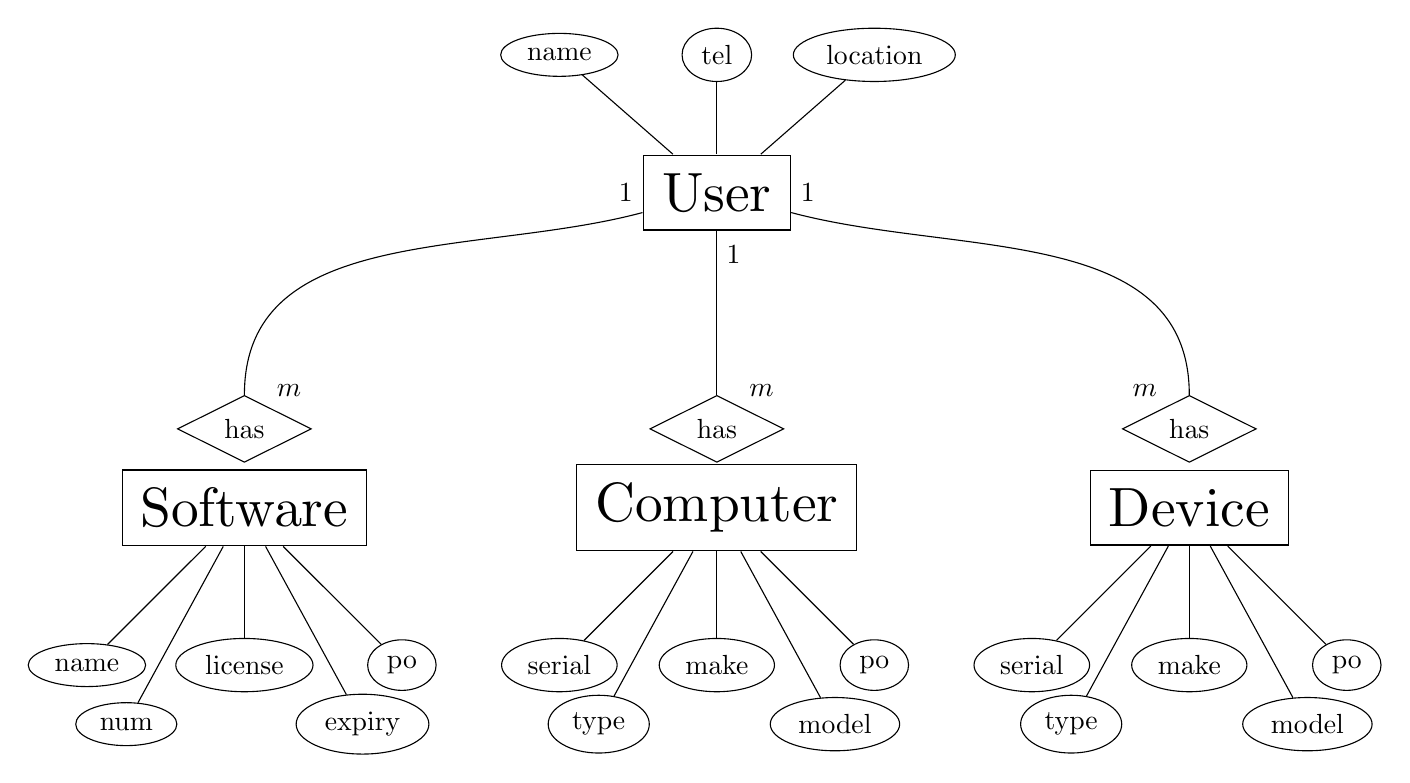
\begin{tikzpicture}[scale=1]
        
                \node at (0,0) [draw, rectangle, scale=2] (computer) {Computer};
                \node at (6,0) [draw, rectangle, scale=2] (device) {Device};
                \node at (-6,0) [draw, rectangle, scale=2] (software) {Software};
                \node at (0,4) [draw, rectangle, scale=2, label=right:{$1$}, label=left:{$1$}] (user) {User};
               
                \node[above of =computer, draw, diamond, aspect=2, label=above right:{$m$}] (has_c) {has};
                \node[above of =device, draw, diamond, aspect=2, label=above left:{$m$}] (has_d) {has};
                \node[above of =software, draw, diamond, aspect=2, label=above right:{$m$}] (has_s) {has};

				\path[] (user) edge[out=270, in =90] node[above right, yshift=.5cm]{$1$} (has_c);
				\path[] (user) edge[out=-15, in =90] (has_d);
				\path[] (user) edge[out=195, in =90] (has_s);
                
                \node[above of =user, draw, ellipse, yshift=.75cm] (u_tel) {tel};
                \node[left of =u_tel, draw, ellipse, xshift=-1cm] (u_name) {name};
                \node[right of =u_tel, draw, ellipse, xshift=1cm] (u_location) {location};
                
                \draw (user) to (u_tel);
                \draw (user) to (u_name);
                \draw (user) to (u_location);
                
                \node[below of= computer, draw, ellipse, yshift=-1cm] (c_make) {make};
                \node[left of= c_make, draw, ellipse, xshift=-1cm] (c_serial) {serial};
                \node[left of= c_make, draw, ellipse, xshift=-.5cm, yshift=-.75cm] (c_type) {type};
                \node[right of= c_make, draw, ellipse, xshift=1cm] (c_po) {po};
                \node[right of= c_make, draw, ellipse, xshift=.5cm, yshift=-.75cm] (c_model) {model};
                
                \draw (computer) to (c_serial);
                \draw (computer) to (c_type);
                \draw (computer) to (c_po);
                \draw (computer) to (c_model);
                \draw (computer) to (c_make);
                
                \node[below of= device, draw, ellipse, yshift=-1cm] (d_make) {make};                
                \node[left of= d_make, draw, ellipse, xshift=-1cm] (d_serial) {serial};
                \node[left of= d_make, draw, ellipse, xshift=-.5cm, yshift=-.75cm] (d_type) {type};
                \node[right of= d_make, draw, ellipse, xshift=1cm] (d_po) {po};
                \node[right of= d_make, draw, ellipse, xshift=.5cm, yshift=-.75cm] (d_model) {model};
                
                \draw (device) to (d_serial);
                \draw (device) to (d_type);
                \draw (device) to (d_po);
                \draw (device) to (d_model);
                \draw (device) to (d_make);                
                
                \node[below of= software, draw, ellipse, yshift=-1cm] (s_license) {license};                
                \node[left of= s_license, draw, ellipse, xshift=-1cm] (s_name) {name};
                \node[left of= s_license, draw, ellipse, xshift=-.5cm, yshift=-.75cm] (s_num) {num};
                \node[right of= s_license, draw, ellipse, xshift=1cm] (s_po) {po};
                \node[right of= s_license, draw, ellipse, xshift=.5cm, yshift=-.75cm] (s_expiry) {expiry};
                
                \draw (software) to (s_name);
                \draw (software) to (s_num);
                \draw (software) to (s_po);
                \draw (software) to (s_expiry);
                \draw (software) to (s_license);                
                
                
%                 \node at (-1, 0) [draw, ellipse] (f_name) {\underline{fname}};
%                 \node at (1, 0) [draw, ellipse] (f_color) {fcolor};
%                 \draw (fans.south west) to (f_name);
%                 \draw (fans.south east) to (f_color);
%                 
%                 %Entity teams(name, color)
%                 \node at (-2,3) [draw, rectangle, scale=2] (teams) {Teams};
%                 \node at (-3, 3.5) [draw, ellipse] (t_name) {\underline{tname}};
%                 \node at (-3, 2.5) [draw, ellipse] (t_color) {tcolor};              
%                 \draw (teams.north west) to (t_name);
%                 \draw (teams.south west) to (t_color);
%                 
%                 %Entity players(name)               
%                 \node at (2,3) [draw, rectangle, scale=2] (players) {Players};
%                 \node at (3, 3.5) [draw, ellipse] (p_name) {\underline{pname}};
%                 \node at (3, 2.5) [draw, ellipse] (is_cap) {is captain};            
%                 \draw (players.north east) to (p_name);
%                 \draw (players.south east) to (is_cap);
%                 
%                 %Relation Player plays_for Team (1-m)
%                 \node at (0,4) [draw, diamond, aspect=2] (plays) {plays for};
%                 \path[] (teams) edge[out=90, in =180] node[below right]{$m$} (plays);
%                 \path[] (plays) edge[out=0, in =90] node[below left]{$1$} (players);
%                 
%                 %Relation Player captains Team (1-1)
%                 \node at (0,2) [draw, diamond, aspect=2] (captains) {captains};
%                 \path[] (teams) edge[out=0, in =180] node[above right]{$1$} (captains);
%                 \path[] (captains) edge[out=0, in =180] node[above left]{$1$} (players);                
%                 
%                 %Relation Fans cheers Team (1-m)
%                 \node at (-2,1.5) [draw, diamond, aspect=2] (cheers_t) {cheers};
%                 \path[] (fans) edge[out=180, in =-90] node[above right]{$1$} (cheers_t);
%                 \path[] (cheers_t) edge[out=90, in =-90] node[above right]{$m$} (teams);                
%                 
%                 %Relation Fans cheers Players (m-m)
%                 \node at (2,1.5) [draw, diamond, aspect=2] (cheers_p) {cheers};
%                 \path[] (fans) edge[out=0, in =-90] node[above left]{$m$} (cheers_p);
%                 \path[] (cheers_p) edge[out=90, in =-90] node[above left]{$m$} (players);                   
                                                
            \end{tikzpicture}
\end{landscape} 
\end{document}
